\section{Simulation}
\label{sec:Simulation}
Die Simulation verfügt über einen Tank, welcher den Pool modelliert, eine Umwälzpumpe und eine Heizung. Des Weiteren wird ein Thermostat zur Temperaturregelung und ein thermisches Netzwerk zur Modellierung der Umgebungseinflüsse eingesetzt.

Um die Simulation übersichtlicher zu Gestalten wurde diese in Teilsysteme unterteilt. Diese werden im nachfolgenden Unterkapitel genauer erläutert. Eine Übersicht des Modells ist in Abbildung \ref{fig:SwimmingPoolSimulationModel} dargestellt.

\vspace{0.5cm}
\begin{figure}[H]
	\centering
	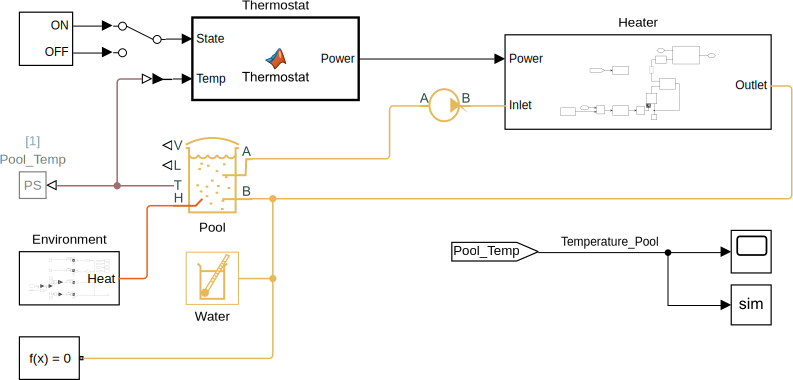
\includegraphics[width=\linewidth]{SwimmingPoolSimulationModel}
	\caption{Simscape-Modell vom Swimmingpool}
	\label{fig:SwimmingPoolSimulationModel}
\end{figure}

\vspace{0.5cm}
\subsection{Teilsysteme}
\label{subsec:Teilsysteme}
Die Simulation verfügt über die folgenden drei Teilsysteme:

\vspace{0.5cm}
\paragraph{Thermostat}
Der Thermostat wurde mit einer MATLAB-Funktion realisiert. Dazu wurde eine \texttt{persistent} Variable verwendet, welche ihren Wert zwischen Funktionsaufrufen beibehält und den Heizzustand speichert. Weiter wird geprüft, ob die aktuelle Temperatur innerhalb eines definierten Bereichs liegt. Dies entspricht einem einfachen Zweipunktregler mit einer Hysterese.

\vspace{0.5cm}
\paragraph{Heizung}
Die Heizung wurde mit einem elektrischen Durchlauferhitzer modelliert. Dazu wird während dem Heizvorgang die entsprechende Spannung an einem Leistungswiderstand angelegt. Die entstehende Wärme wird dann über ein 0.5\,m langes Kupferrohr mit einem Durchmesser von 10\,cm durch Wärmeleitung in das Wasser übertragen. Die Leistung des Durchlauferhitzers entspricht der berechneten Leistung der Wärmepumpe (siehe \ref{subsec:Annahmen}). Abbildung \ref{fig:HeaterModel} zeigt das Teilsystem.

\begin{figure}[H]
	\centering
	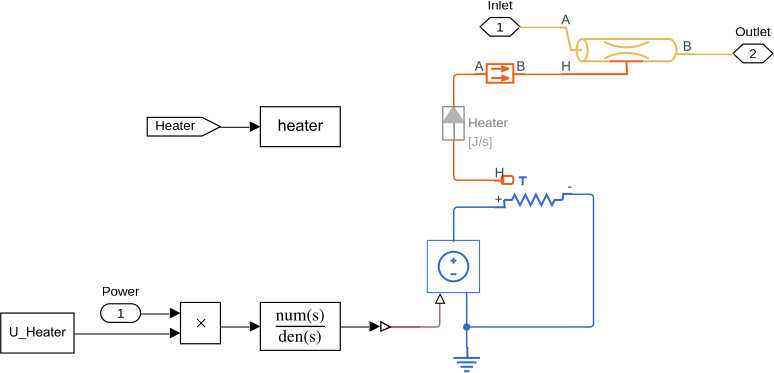
\includegraphics[width=\linewidth]{HeaterModel}
	\caption{Teilsystem: Heizung}
	\label{fig:HeaterModel}
\end{figure}

\vspace{0.5cm}
\paragraph{Umgebung}
Die Umwelt beeinflusst mit vier verschiedene Faktoren die Pooltemperatur:

\begin{itemize}
	\item Temperaturzunahme / -abnahme durch Wärmeleitung (Poolwände)
	\item Temperaturzunahme / -abnahme durch Konvektion (Wasser zu Luft)
	\item Temperaturabnahme durch Wasserverdunstung
	\item Temperaturzunahme durch die Sonnenstrahlen
\end{itemize}

Diese vier Faktoren befinden sich im Teilsystem \texttt{Environment} und sind parallel geschaltet. Das Vorgehen der vier Blöcke ist immer ähnlich. Es wird jeweils ein mathematisches Signal beschrieben, welches am Ende mit einem \texttt{PS-Converter} in die physikalische Umgebung übersetzt wird. Dieses Temperatur- oder Leistungssignal kontrolliert dann eine ideale Energiequelle.

Die Wasserverdunstung hängt hauptsächlich von der Sonne ab und macht einen grossen Anteil der Verluste aus \cite{WasserVerdunsten}. Deshalb erfolgt der Wärmeverlust entsprechend der Funktion der Sonnenstrahlung. Dabei wird dem Pool mit dem Simscape-Element \texttt{Controlled Heat Flow Rate Source} Energie entzogen. Die Energiemenge wurde mithilfe der Arbeitsgrundlagen (siehe Kapitel \ref{subsec:Annahmen}) berechnet und der mittlere Wert der Funktion entsprechend gewählt. Um einen Verlust zu erreichen, besitzt die Funktion ein negatives Vorzeichen.

Die Sonneneinstrahlung wird gleich implementiert, wie die Wasserverdunstung. Die Funktion ist jedoch positiv, was zu einer Energiezufuhr führt. Ausserdem besitzt die Funktion eine andere Amplitude, welche der Sonnenenergie entspricht.

Um die Wärmeverluste / -gewinne durch den Boden zu simulieren, bietet Simscape das Element \texttt{Thermal Resistance}. Dazu wird auf beiden Seiten eine Wärmequelle angeschlossen sowie der thermische Widerstand spezifiziert. Simscape simuliert dann den Wärmefluss in J/s, welcher proportional zur Temperaturdifferenz ist. Ausserdem wird das Element \texttt{Controlled Temperature Source} verwendet, welches eine ideale Energiequelle darstellt.

Mit dem Element \texttt{Convective Heat Transfer} können die Konvektionsverluste simuliert werden. Wie beim Boden wird auf beiden Seiten des Elements eine Wärmequelle angeschlossen. Das Element benötigt zusätzlich noch die Pooloberfläche sowie den Wärmeübergangskoeffizienten.

Abbildung \ref{fig:EnvironmentModel} zeigt das Teilsystem, welches die Umwelteinflüsse modelliert:

\begin{figure}[H]
	\centering
	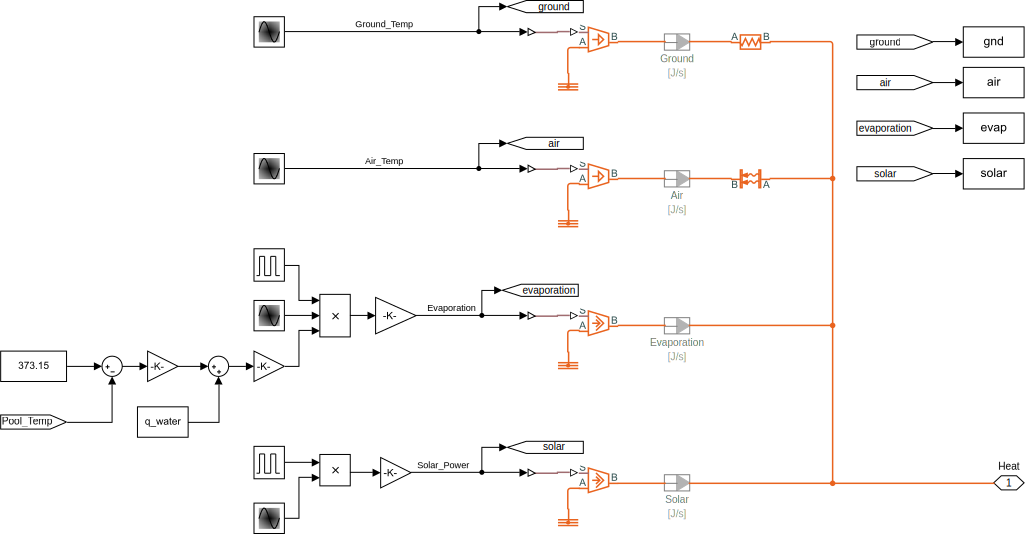
\includegraphics[width=\linewidth]{EnvironmentModel}
	\caption{Teilsystem: Umgebung}
	\label{fig:EnvironmentModel}
\end{figure}
